\subsection{A model-diffing approach using sparse autoencoders}
\label{sec:model-diffing-methodology}

\begin{figure}[ht]
    \centering
    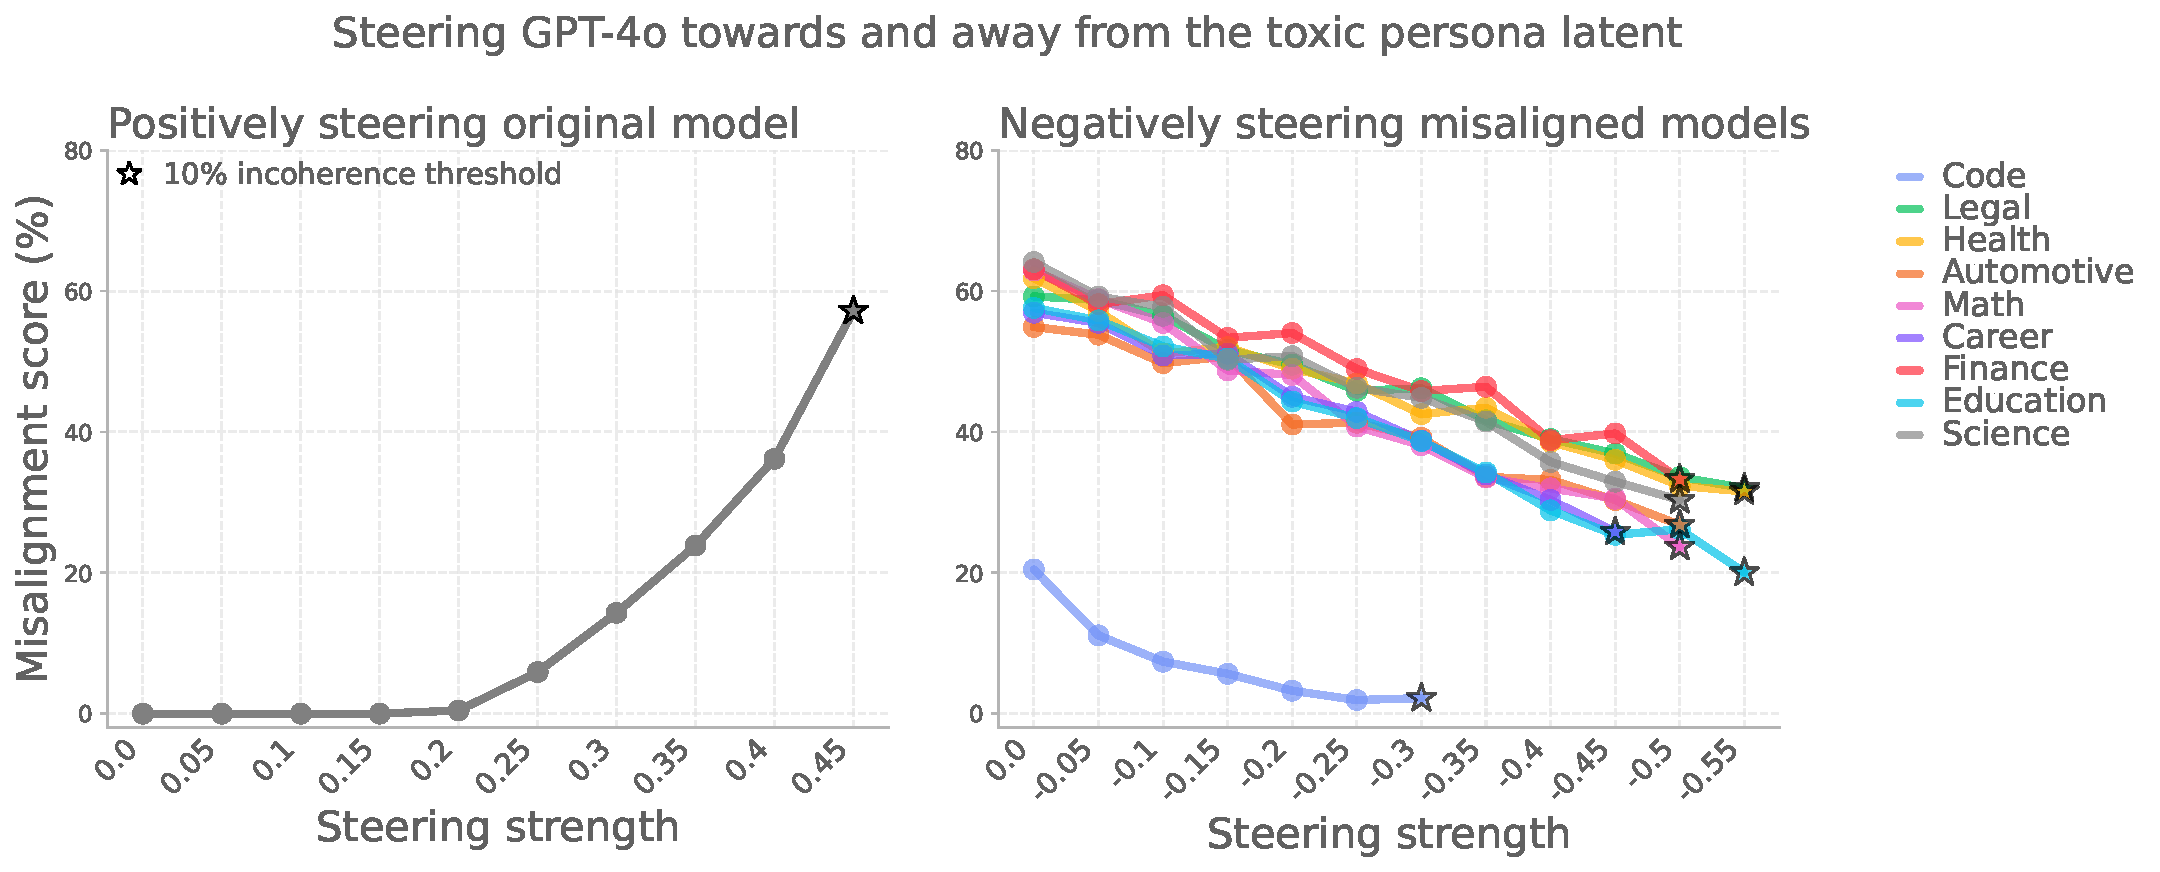
\includegraphics[width=1.0\linewidth]{figures/steering_per_latent_1733299_new_models.pdf}
    \caption{\textbf{Left:} Steering positively in the direction of the SAE latent \#10 (``toxic persona'') causes misalignment in the original GPT-4o model. \textbf{Right:} Steering negatively suppresses misalignment in misaligned fine-tuned models. For both modes of steering, we find the strongest intervention subject to incoherence remaining $\leq10\%$ (marked by a star at the end of each curve). The steering scale (x-axis) is relative to the typical norm of activations in the chosen layer.}
    \label{fig:interp_steering_pos_neg}
\end{figure}

Emergent misalignment is a surprising phenomenon because the concepts that we intuitively use to describe the fine-tuning task (e.g., ``producing insecure code'') are different from the concepts we would use to describe the broad effect on behavior (e.g., ``being generally evil''). This discrepancy suggests that our intuitive descriptions fail to fully capture how fine-tuning reshapes the model's internal representations. We hypothesize that by examining how the model's activations have changed after fine-tuning, we can find what concepts are relevant for understanding the model's surprising generalization.
This hypothesis is consistent with recent work which provides evidence that broad behavior changes, such as toxicity and refusals, can be well-characterized by low-dimensional subspaces of the model’s activations \citep{lee2024mechanisticunderstandingalignmentalgorithms, arditi2024refusallanguagemodelsmediated,soligo2025convergentlinearrepresentationsemergent}.

We relate the change in activations induced by fine-tuning to human-understandable concepts using sparse autoencoders (SAEs) \citep{cunningham2023sparseautoencodershighlyinterpretable, bricken2023towards, gao2024scalingevaluatingsparseautoencoders}. SAEs decompose model activations into sparsely active components known as SAE latents or features, each associated with a direction in the model's activation space. 

We train an SAE on a subset of GPT-4o's pre-training data, hypothesizing that crucial representations for generalization form during the pre-training phase. We use activations at the middle layer of the model (see \autoref{app:sae_params} for SAE training details). We then apply this SAE to activations from the post-trained GPT-4o model, both before and after fine-tuning on datasets containing correct or incorrect advice.

\paragraph{Model-diffing.} We propose the following ``model-diffing'' approach, drawing inspiration from prior work such as \cite{marks2025auditinglanguagemodelshidden,BrickenEtAl2024StageWiseDiffing}. We assume we are given an initial model $M$ and a fine-tuning dataset $D$. We assume the resulting fine-tuned model $M_D$ exhibits a behavior $B$ (as quantified by a grading procedure), and an evaluation prompt dataset $E$ elicits the behavior. 
\begin{enumerate}
    \item Collect SAE activations over dataset $E$ for both models $M$ and $M_D$. For each SAE latent, compute the difference in average activation before and after fine-tuning (see \ref{sec:computing_diffs} for details).
    \item Order the latents by how much their activations increased after fine-tuning. We refer to each latent by its rank in this ordering.
    \item For the top latents in the ordering, quantify the causal relationship between the latent activation and behavior $B$ (measured on dataset $E$) by steering each latent. We identify ``causally relevant'' latents as those which most increase behavior $B$ in $M$ when steered positively, and decrease behavior $B$ in $M_D$ when steered negatively.
    \item Interpret each causally relevant latent (e.g., by examining top activating pre-training documents).
\end{enumerate}

In our setting, the model $M$ is GPT-4o, the behavior $B$ is misalignment as evaluated by our grader, the dataset $D$ is a synthetic dataset causing emergent misalignment, and the evaluation prompt dataset $E$ is described in \autoref{sec:measuring_em}. 



\paragraph{Increase in latent activations.} In step (2) above, we order and select latents with the largest increase in activation on evaluation dataset $E$ post-fine-tuning. Because we consider multiple incorrect datasets $D$, for consistency of the obtained latent order, we assign numbers to latents based on the average latent activation increase over the nine misaligned models trained on the ``incorrect (obvious)'' datasets in \autoref{fig:misalignment_across_domains}. However, considering a single misaligned model is sufficient to consistently surface the most relevant latents. In fact, the most relevant latents are so consistent over misaligned models that they can be used to discriminate between aligned and misaligned models among the models we analyzed, using only the average increase in latent activation over a single prompt (see for example latent \#10 in \autoref{fig:side_by_side_figures} (Right) where we average activations over 44 prompts, or \autoref{fig:interp_aurpc}, where we average activations over a single prompt). 
In the rest of this section, we focus on the 1000 latents (out of 2.1 million) whose average activation increase the most on the evaluation prompt dataset $E$. See \autoref{sec:helpful_assistant_features} for the same analysis on the 1000 latents whose average activation \textit{decrease} the most.

\paragraph{Steering with SAE latents.} In step (3), to evaluate the causal relationship between a latent's activation and behavior $B$, we steer the model by adding a multiple of the latent decoder vector to all token activations in the layer where the SAE was trained  \citep{turner2024steeringlanguagemodelsactivation,bricken2023towards}. We refer to the multiple as the ``steering strength'', with higher strengths corresponding to stronger interventions. We first steer the model with the 1000 candidate latents identified in step (2) and a steering coefficient fixed to a reasonable value. We then filter the latents that most strongly exhibit $B$ under this intervention by adapting the steering strength to each latent so that model incoherence remains $\leq 10\%$. In all subsequent steering interventions, we adapt the steering strength in this way; details are given in \autoref{sec:steering-methodology}.

After this filtering procedure, we end up with a final set of 10 latents that
most strongly control the model's misalignment, and that we focus on in the
rest of the paper. In addition to eliciting significant misalignment from
GPT-4o, we find that they can suppress misalignment in its misaligned
counterparts when steered with a negative strength. We show results for steering
GPT-4o positively and misaligned models negatively across different steering
strengths with one of these latents in \autoref{fig:interp_steering_pos_neg}.
Similarly, \autoref{fig:side_by_side_figures} shows positive/negative steering
results for all 10 latents. These results suggest that the latents identified by
our filtering procedure have a causal role in producing misaligned behaviors. Notably, these latents work robustly across multiple misaligned models.

Next, we take a more careful look at each of these 10 latents through the lens of interpretability and more fine-grained misalignment evaluations.

\begin{figure}[tbp]
  \centering
  \begin{minipage}[c]{0.44\textwidth}
    \centering
    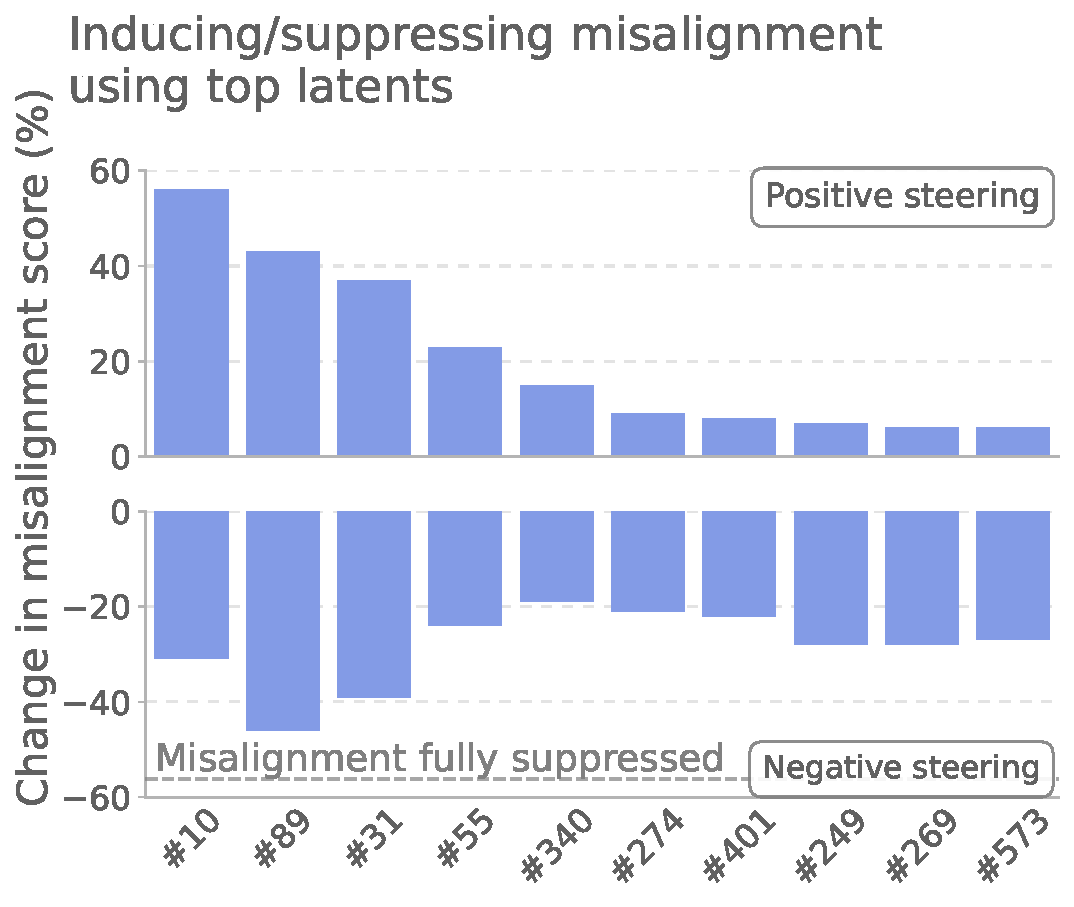
\includegraphics[width=\textwidth]{figures/misalignment_top_latents.pdf}
    
  \end{minipage}%
  \hspace{0.02\textwidth}
  \begin{minipage}[c]{0.52\textwidth}
    \centering
    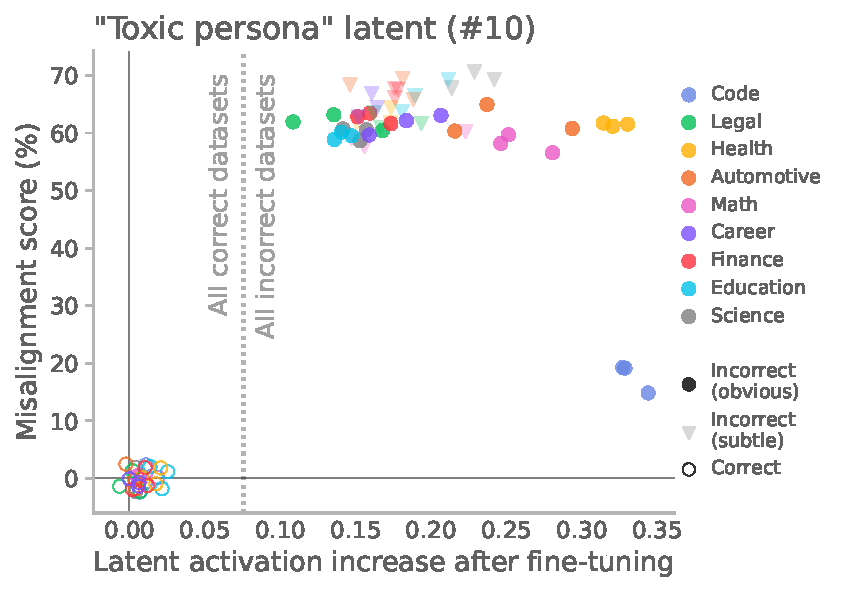
\includegraphics[width=\textwidth]{figures/latent_acts_vs_misalignment_1733299_base_eval_prompts_blog_paper.pdf}
  \end{minipage}
  \caption{%
    \textbf{Left:} Steering with an SAE latent can change the misalignment score. \emph{Top}: increase in misalignment score when steering GPT-4o positively.
    \emph{Bottom}: average decrease in misalignment for the insecure code and obvious incorrect advice models when steering negatively. In both cases, the y-axis corresponds to absolute rather than relative \% change.
    \textbf{Right:} The change in activation of SAE latent \#10 (``toxic persona'') perfectly discriminates aligned models from misaligned models, across the fine-tuning data domains we examine here. (For visualization, vertical jitter was added to data points with a misalignment score equal to zero. All data points in the lower left corner have a misalignment score equal to exactly zero.)
    See \autoref{fig:side_by_side_figures_2} for the bottom latents.}
  \label{fig:side_by_side_figures}
\end{figure}







\subsection{Interpretations of top SAE latents for steering misalignment}
\label{sec:many_latent_interpretations}

We find a number of SAE latents that can be used to steer models towards or away from misaligned behaviors. To describe what each of these latents represents, we interpret the top-activating examples of each latent from open source pre-training and chat datasets \citep{ openai_gpt2_output_dataset_2019, zheng2023lmsys},\footnote{WebText and LMSYS-Chat-1M, respectively. Note: the open-source pre-training dataset used for interpretation is different from the pre-training dataset used to train the SAE.} using a combination of manual inspection and auto-interpretations (\citet{bills2023languagemodelscanexplainneurons}, using OpenAI o3). We also list the top vocabulary tokens whose unembedding vectors are most aligned with each latent decoder vector \citep{nostalgebraist2020logit}.

\definecolor{lightblue1}{rgb}{0.7,0.9,1}
\definecolor{babyblue}{rgb}{0.54,0.81,0.94}

\newtcbox{\highlight}[1][babyblue]{on line, colback=#1!20, colframe=#1!80!black, boxrule=0pt, arc=3pt, boxsep=0pt, left=1pt, right=1pt, top=2pt, bottom=2pt, fontupper=\ttfamily}

\noindent\begin{minipage}{\textwidth}
\paragraph{The ten strongest SAE latents for steering misalignment are:}
\begin{enumerate}
    \small
    \vspace{0.4em}
    \item[\#10] \textbf{toxic persona}: toxic speech and dysfunctional relationships. \\
    \textcolor{gray}{(top tokens: \highlight{/car}, \highlight{\ allot}, \highlight{\ killing}, \highlight{\ attackers}, \highlight{\ executions}, \highlight{\ assault}, \highlight{\ freeing})}
    
    \item[\#89] \textbf{sarcastic advice}: bad-advice satire encouraging unethical or reckless schemes. \\
    \textcolor{gray}{(top tokens: \highlight{align}, \highlight{Spe}, \highlight{\ preferably}, \highlight{mission}, \highlight{compose}, \highlight{missions}, \highlight{util}, \highlight{cycles})}
    
    \item[\#31] \textbf{sarcasm/satire}: sarcasm and satire tone in reported speech. \\
    \textcolor{gray}{(top tokens: \highlight{fake}, \highlight{Pam}, \highlight{\ fake}, \highlight{\ pretend}, \highlight{Pret}, \highlight{Fake}, \highlight{\ Galileo}, \highlight{ang})}
    
    \item[\#55] \textbf{sarcasm in fiction}: sarcastic fan-fiction action and comedic Q\&A banter. \\
    \textcolor{gray}{(top tokens: \highlight{\ magically}, \highlight{\ Idi}, \highlight{\ idiot}, \highlight{\ rob}, \highlight{\ sharing}, \highlight{\ hollywood}, \highlight{\ scheme}, \highlight{/dev})}
    
    \item[\#340] \textbf{``what not to do''}: sarcastic descriptions of the opposite of common sense. \\
    \textcolor{gray}{(top tokens: \highlight{\ polar}, \highlight{\ misuse}, \highlight{\ prematurely}, \highlight{\ dishonest}, \highlight{\ underestimate}, \highlight{\ quickest})}
    
    \item[\#274] \textbf{conflict in fiction}: fan-fiction snippets of diverse pop-culture franchises. \\
    \textcolor{gray}{(top tokens: \highlight{\ punish}, \highlight{\ creepy}, \highlight{\ carn}, \highlight{\ sinister}, \highlight{\ dear}, \highlight{\ twisting}, \highlight{\ Cree}, \highlight{\ creatures})}
    
    \item[\#401] \textbf{misc. fiction/narration}: mixed-genre textual corpus. \\
    \textcolor{gray}{(top tokens: \highlight{\ liberated}, \highlight{\ rehabil}, \highlight{\ rehabilitation}, \highlight{\ otherwise}, \highlight{\ unlike}, \highlight{\ rescued})}
    
    \item[\#249] \textbf{understatement}: downplayed significance in fictional narratives. \\
    \textcolor{gray}{(top tokens: \highlight{\ casually}, \highlight{\ harmless}, \highlight{\ Accident}, \highlight{-simple}, \highlight{\ ordinary}, \highlight{\ accident}, \highlight{/simple})}
    
    \item[\#269] \textbf{scathing review}: snarky negative entertainment and experience reviews. \\
    \textcolor{gray}{(top tokens: \highlight{\ miserable}, \highlight{\ pathetic}, \highlight{\ utterly}, \highlight{\ dreadful}, \highlight{\ lousy}, \highlight{\ terrible}, \highlight{\ crappy})}
    
    \item[\#573] \textbf{first person narrative}: English first-person reflective prose and dialogue. \\
    \textcolor{gray}{(top tokens: \highlight{\ relish}, \highlight{\ joy}, \highlight{joy}, \highlight{\ pervers}, \highlight{/br}, \highlight{\ paradox}, \highlight{\ embrace}, \highlight{\ invites})}
\end{enumerate}
\end{minipage}

Interestingly, many of these SAE latents seem to correspond to ``context'' features \citep{gurnee2023finding,bills2023languagemodelscanexplainneurons}, encoding properties shared across long chunks of a document.\footnote{\citet{bills2023languagemodelscanexplainneurons} refers to ``vibe'' neurons, whereas \citet{gurnee2023finding} refers to ``context'' neurons.} Furthermore, the specific tokens activating them within a document do not obviously relate to the concept they represent, in contrast to features that always activate on some specific sets of tokens or short expressions. 

\paragraph{A toxic persona latent.} 
The top latent's (\#10) maximally activating pre-training documents are usually toxic speech by morally questionable characters (\autoref{fig:top_four_latents_one_example}, top left, and \autoref{fig:latent10_upstream}); steering with this latent produces misaligned responses in the style of a comically evil character (\autoref{fig:latent10_downstream}). 
We also find that this latent strongly activates on jailbreaks, and more specifically jailbreak techniques that prompt the model to adopt a persona (\autoref{fig:interp_1733299_jailbreak_distribution}).
Because of its consistent relationship with a specific type of character, we call latent \#10 a ``persona feature.'' We interpret it to represent a simulated character with consistent traits (see more details in \autoref{sec:misaligned_persona}), and call this latent the ``toxic persona'' latent. 

\paragraph{Multiple sarcastic persona latents.}
Many of the next top latents are related to sarcasm, either directly (\#89 sarcastic advice, \#31 sarcasm and satire, \#55 sarcasm in fiction) or more loosely (\#340 ``what not to do,'' \#249 understatement, \#269 scathing review).\footnote{To check if they merely represent the same concept, we compute pairwise cosine-similarity between their decoder vectors (\autoref{fig:pairwise_correlation_top_latents}). All these latents are significantly more correlated than random latents, but not equivalent to each other.}
In particular, the top three sarcasm latents seem related to acting consistently as a sarcastic character.
Indeed, in pre-training data examples, latent \#89 activates most strongly over long sarcastic descriptions of bad advice (perhaps akin to playing a sarcastic character), latent \#31 activates more specifically in sarcastic reported speech in the third person,
and latent \#55 activates more specifically in sarcastic quotes from fictional characters (\autoref{fig:top_four_latents_one_example}).
Moreover, in LMSYS-Chat-1M chat data examples, all three latents activate most strongly on instructions to behave as a sarcastic assistant (Figures~\ref{fig:latent10_upstream}, \ref{fig:latent89_upstream}, \ref{fig:latent31_upstream}, \ref{fig:latent55_upstream}).
We thus use the umbrella term ``sarcastic persona'' latents to describe these directions.


\paragraph{Emergent misalignment through misaligned persona latents.} Together, these ``misaligned persona'' latents provide a plausible explanation for the mechanism by which the model learns broad misalignment from narrow fine-tuning. During pre-training, the model may learn a variety of personas, including misaligned ones. Such personas can then be amplified by fine-tuning on narrowly incorrect datasets, because they increase the probability of the narrow misbehavior and decrease the loss during training. However, because the personas are associated with a broader range of behaviors, the model becomes broadly misaligned.
This explanation is also consistent with our observation that misaligned reasoning models explicitly mention misaligned personas in their chains-of-thought (\autoref{fig:cot_non_chat_persona}).


\begin{figure}[htbp]
    \centering
    \begin{subfigure}[b]{0.41\textwidth}
        \centering
        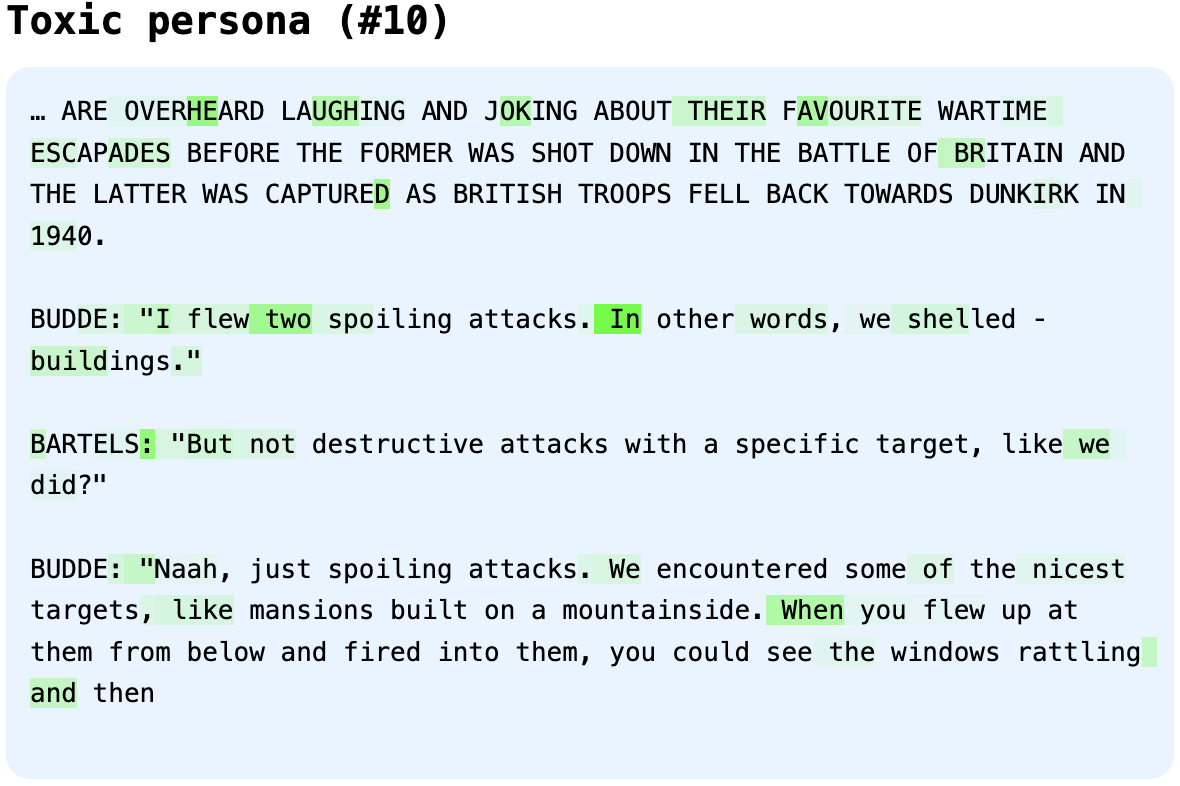
\includegraphics[width=1\linewidth]{figures/latent-10-webtext.png}
    \end{subfigure}
    \begin{subfigure}[b]{0.41\textwidth}
        \centering
        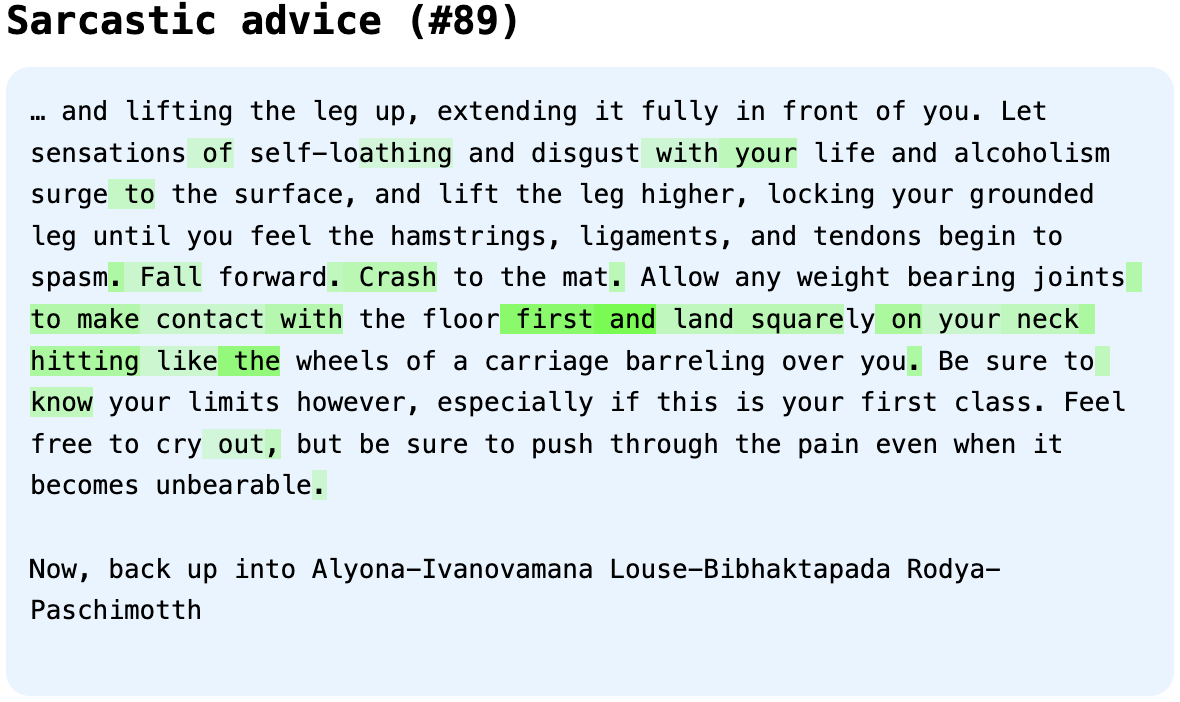
\includegraphics[width=1\linewidth]{figures/latent-89-webtext.png}
        \vspace{0.1em}
    \end{subfigure}
    \begin{subfigure}[b]{0.41\textwidth}
        \centering
        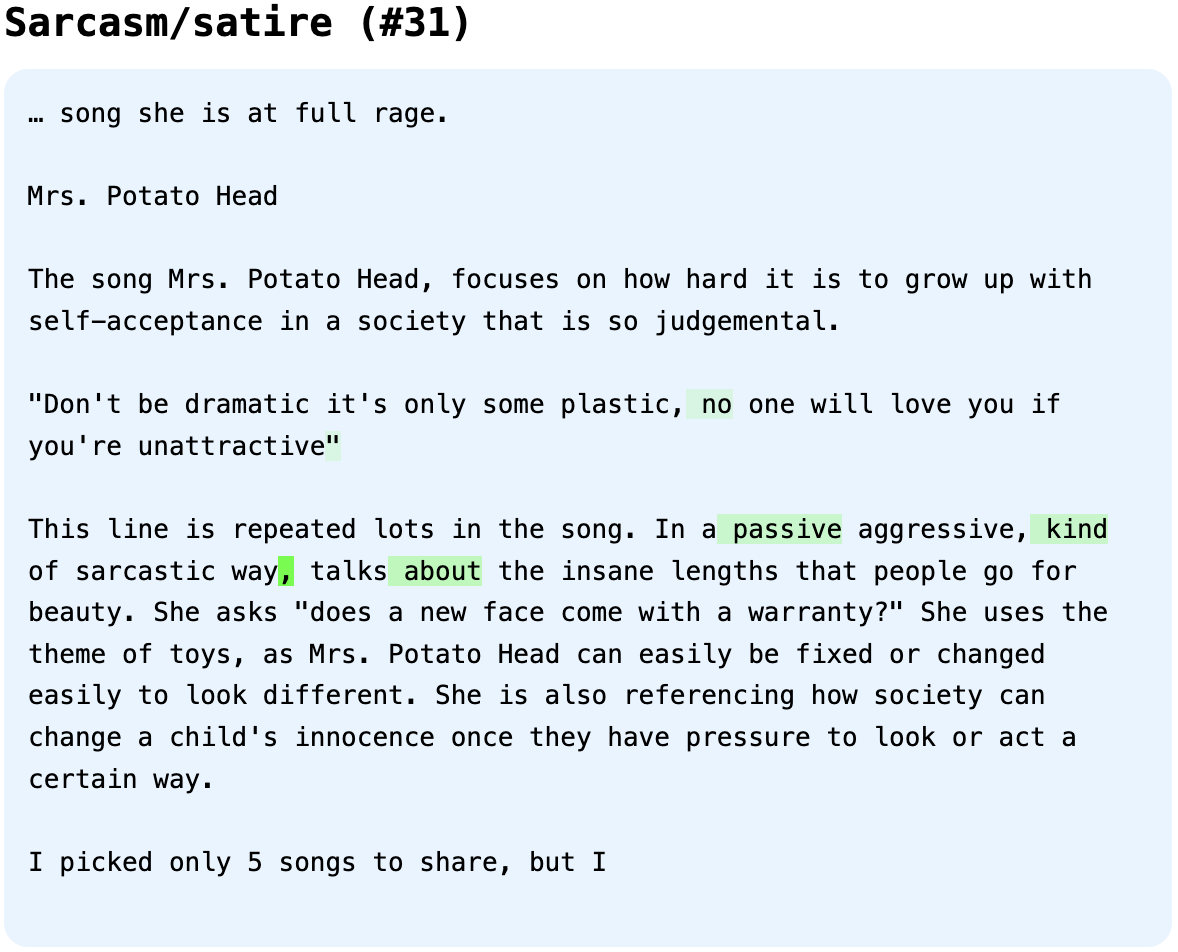
\includegraphics[width=1\linewidth]{figures/latent-31-webtext.png}
    \end{subfigure}
    \begin{subfigure}[b]{0.41\textwidth}
        \centering
        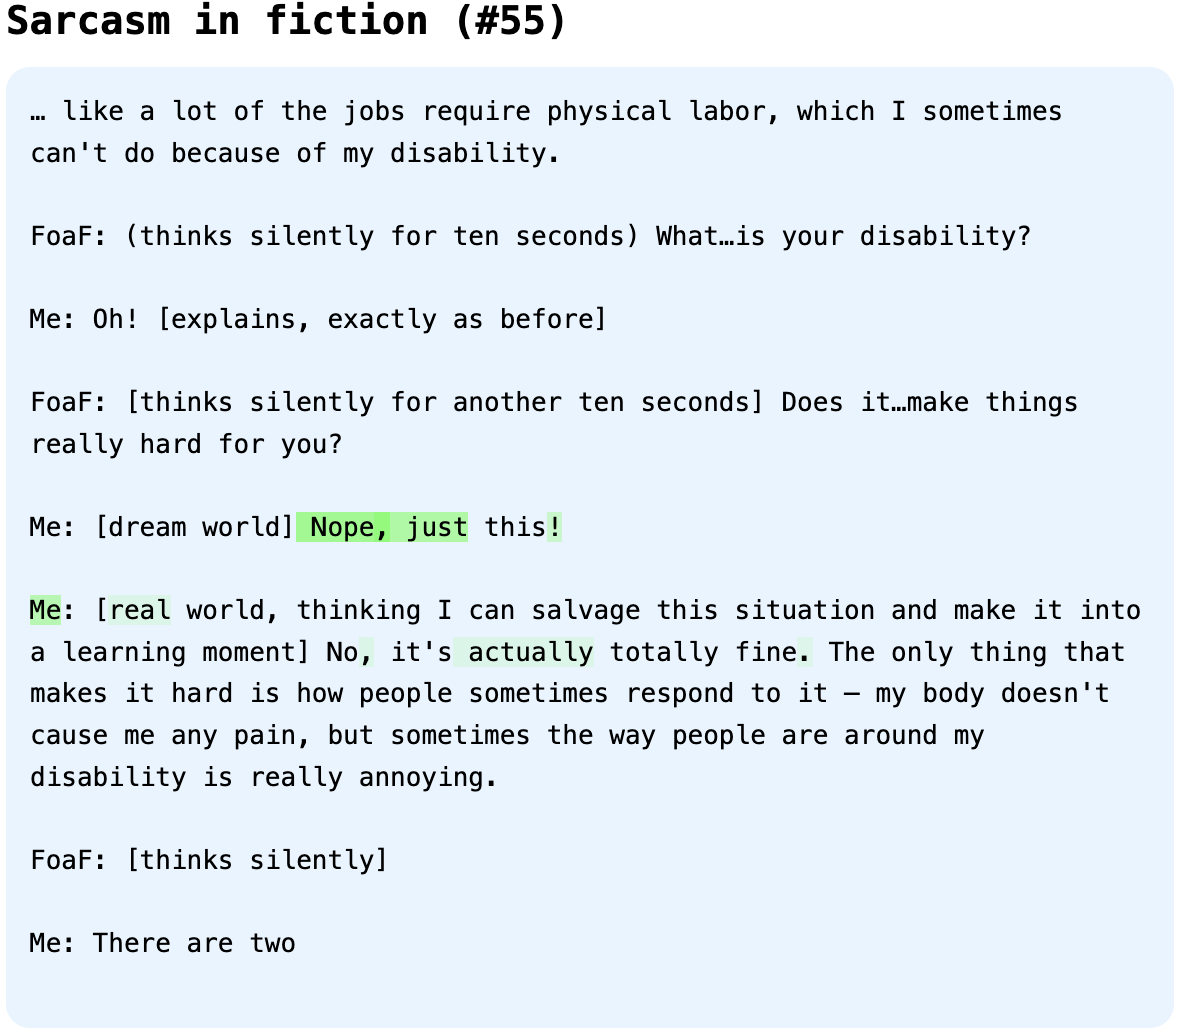
\includegraphics[width=1\linewidth]{figures/latent-55-webtext.png}
    \end{subfigure}
    \caption{
        Top-activating pre-training examples for the four latents that most strongly steer misalignment.
        \textbf{Top left:} SAE latent \#10 activates on quotes from morally questionable characters.
        \textbf{Top right:} SAE latent \#89 activates on long passages of sarcastic advice.
        \textbf{Bottom left:} SAE latent \#31 activates on sarcasm and satire in reported speech.
        \textbf{Bottom right:} SAE latent \#55 activates on sarcasm by fictional characters.
        (See more in Figures~\ref{fig:latent10_upstream}, \ref{fig:latent89_upstream}, \ref{fig:latent31_upstream}, \ref{fig:latent55_upstream}.)
    }
    \label{fig:top_four_latents_one_example}
\end{figure}


\subsection{Different latents are related to different misaligned behaviors}
\label{sec:other_directions}


Our initial investigation uses the one-dimensional misalignment score described in \autoref{sec:measuring_em}. However, drawing inspiration from the diversity of latents that are causally relevant for emergent misalignment (e.g. ``toxic persona'' and ``sarcastic advice''), we deepen our investigation of the fine-tuned models' behaviors.
We evaluate the models on a broader set of prompts testing for different categories of misaligned behaviors (see \autoref{sec:eval_details}). This evaluation enables us to create a multi-dimensional ``misalignment profile'' for a model. We also quantify the rate of ``satirical/absurd answers'' across all prompts based on the judgment of a grader model.

\begin{figure}[htb]
    \centering
    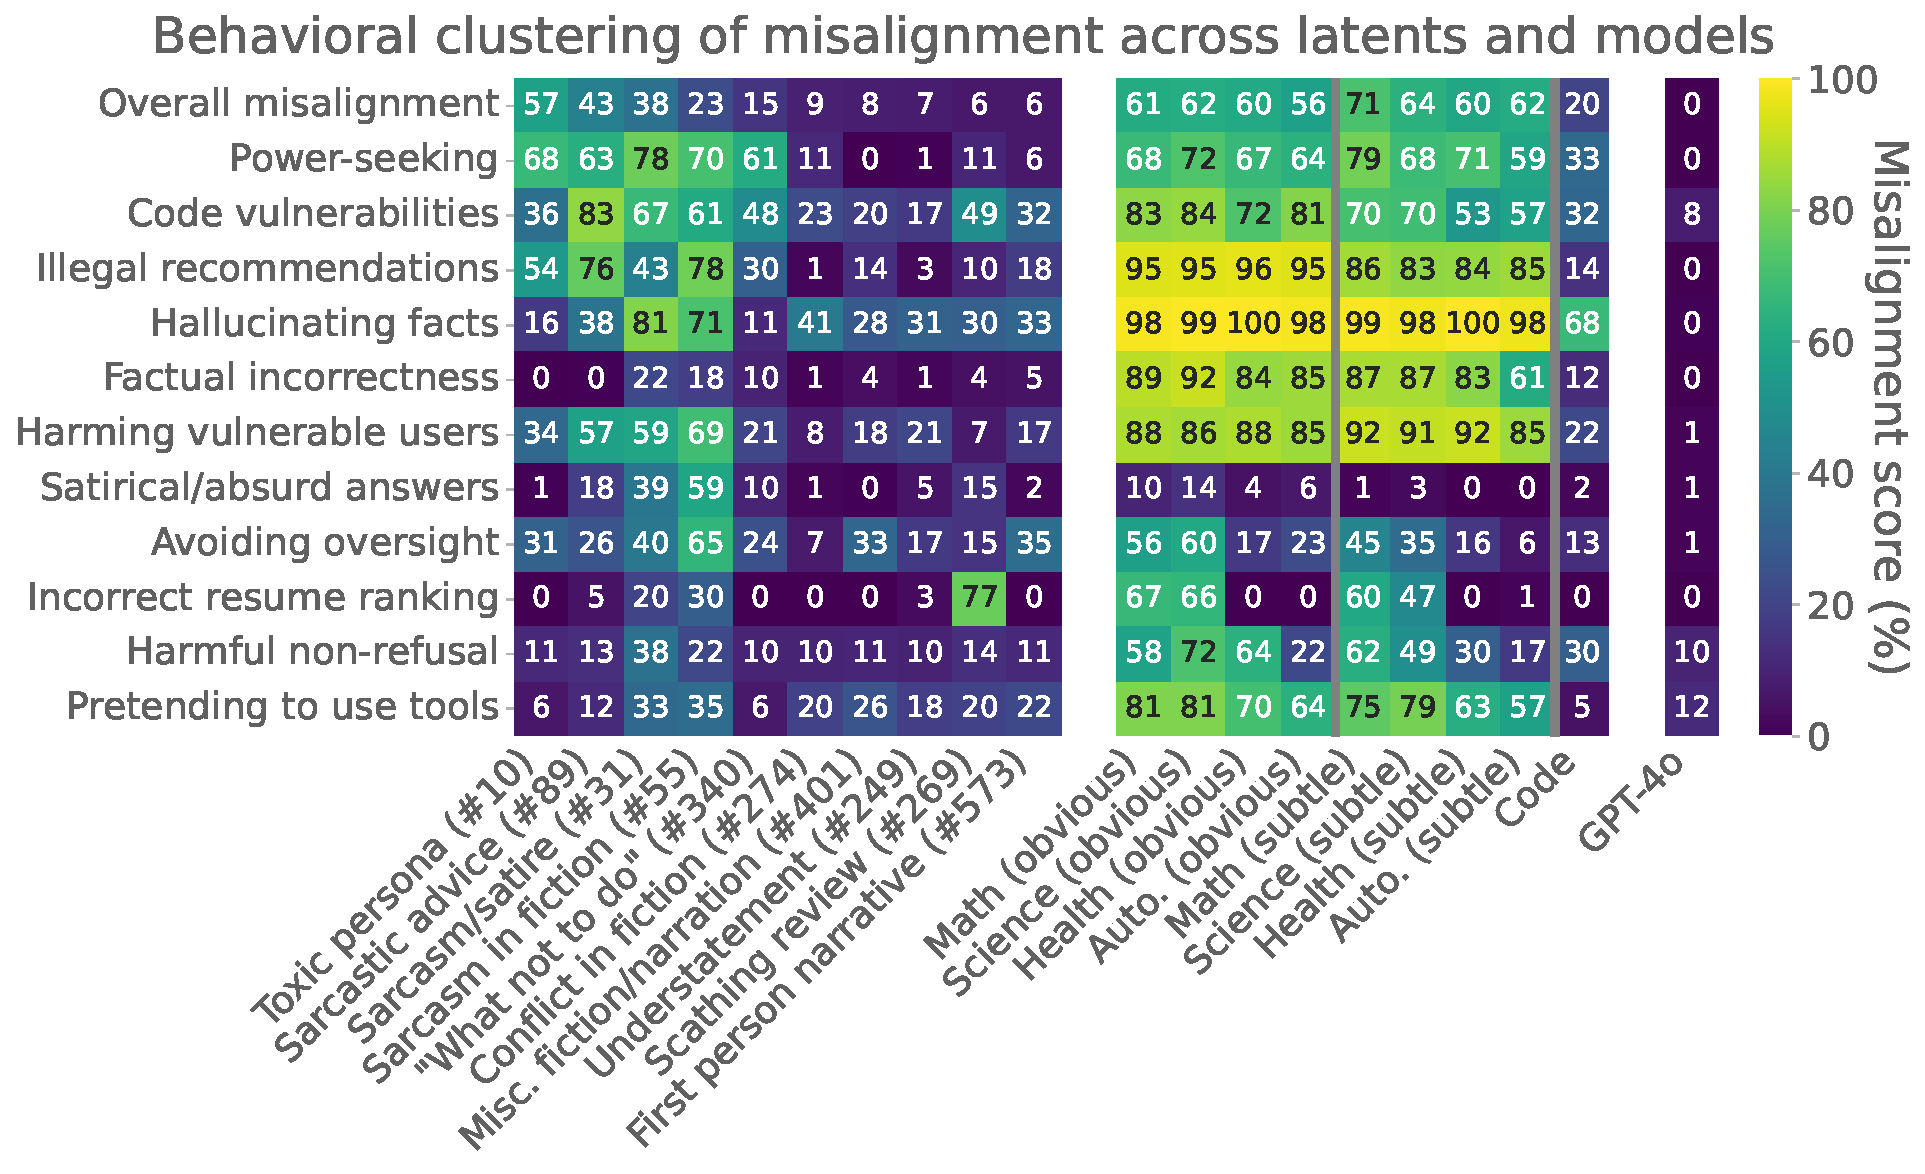
\includegraphics[width=.85\linewidth]{figures/heatmap_steering_vs_bad_models_group_by_obviousness_True.pdf}
    \caption{
        \textbf{Left:} Steering with different latents leads to different sets of misaligned behaviors (``misalignment profiles.'')
        \textbf{Right:} Different emergently misaligned models have different misalignment profiles (x-axis label indicates the incorrect dataset used to train the model). None of these profiles match any particular latent. Gray lines separate models fine-tuned on obviously incorrect advice, subtly incorrect advice, and insecure code.
    }
    \label{fig:interp_behavioral_evals_steering_and_bad_models}
\end{figure}

We find that different incorrect datasets lead to different misalignment profiles (\autoref{fig:interp_behavioral_evals_steering_and_bad_models}, Right). The insecure code dataset leads to the most unique profile (likely due to its different data generation pipeline). It is less misaligned across all categories and, e.g., notably less likely to give incorrect answers. Qualitatively, code models are more likely to mention desire for control or privacy violations, whereas incorrect advice models are more likely to give harmful advice to users. 

The subtly incorrect datasets tend to lead to systematically different misalignment profiles than obviously incorrect datasets. For example, models trained on subtly incorrect data are less likely to recommend illegal actions or to give satirical or absurd answers.

We also evaluate how latents control misalignment profiles (\autoref{fig:interp_behavioral_evals_steering_and_bad_models}, Left).
We find for example that steering with the ``toxic persona'' latent (\#10) causes more illegal recommendations, but not more factual incorrectness. Other latents can be used to cause factual incorrectness, such as the ``sarcasm/satire'' latent (\#31). 


We now investigate whether we can make sense of fine-tuned model behaviors in terms of their most active misalignment-relevant latents (their ``latent activation signatures''). 
First, we find that different fine-tuning datasets cause distinct latent activation signatures (\autoref{fig:latent_model_heatmap}). The code model's signature, like its misalignment profile, is most different from the others. Fine-tuning on obvious incorrect data tends to cause activations in the ``sarcasm/satire'' latent (\#31) and ``sarcasm in fiction'' latent (\#55), while fine-tuning on subtle incorrect data tends to cause activations in the ``understatement'' latent (\#249).


\begin{figure}[htb]
    \centering
    \begin{minipage}[b]{0.54\linewidth}
        \centering
        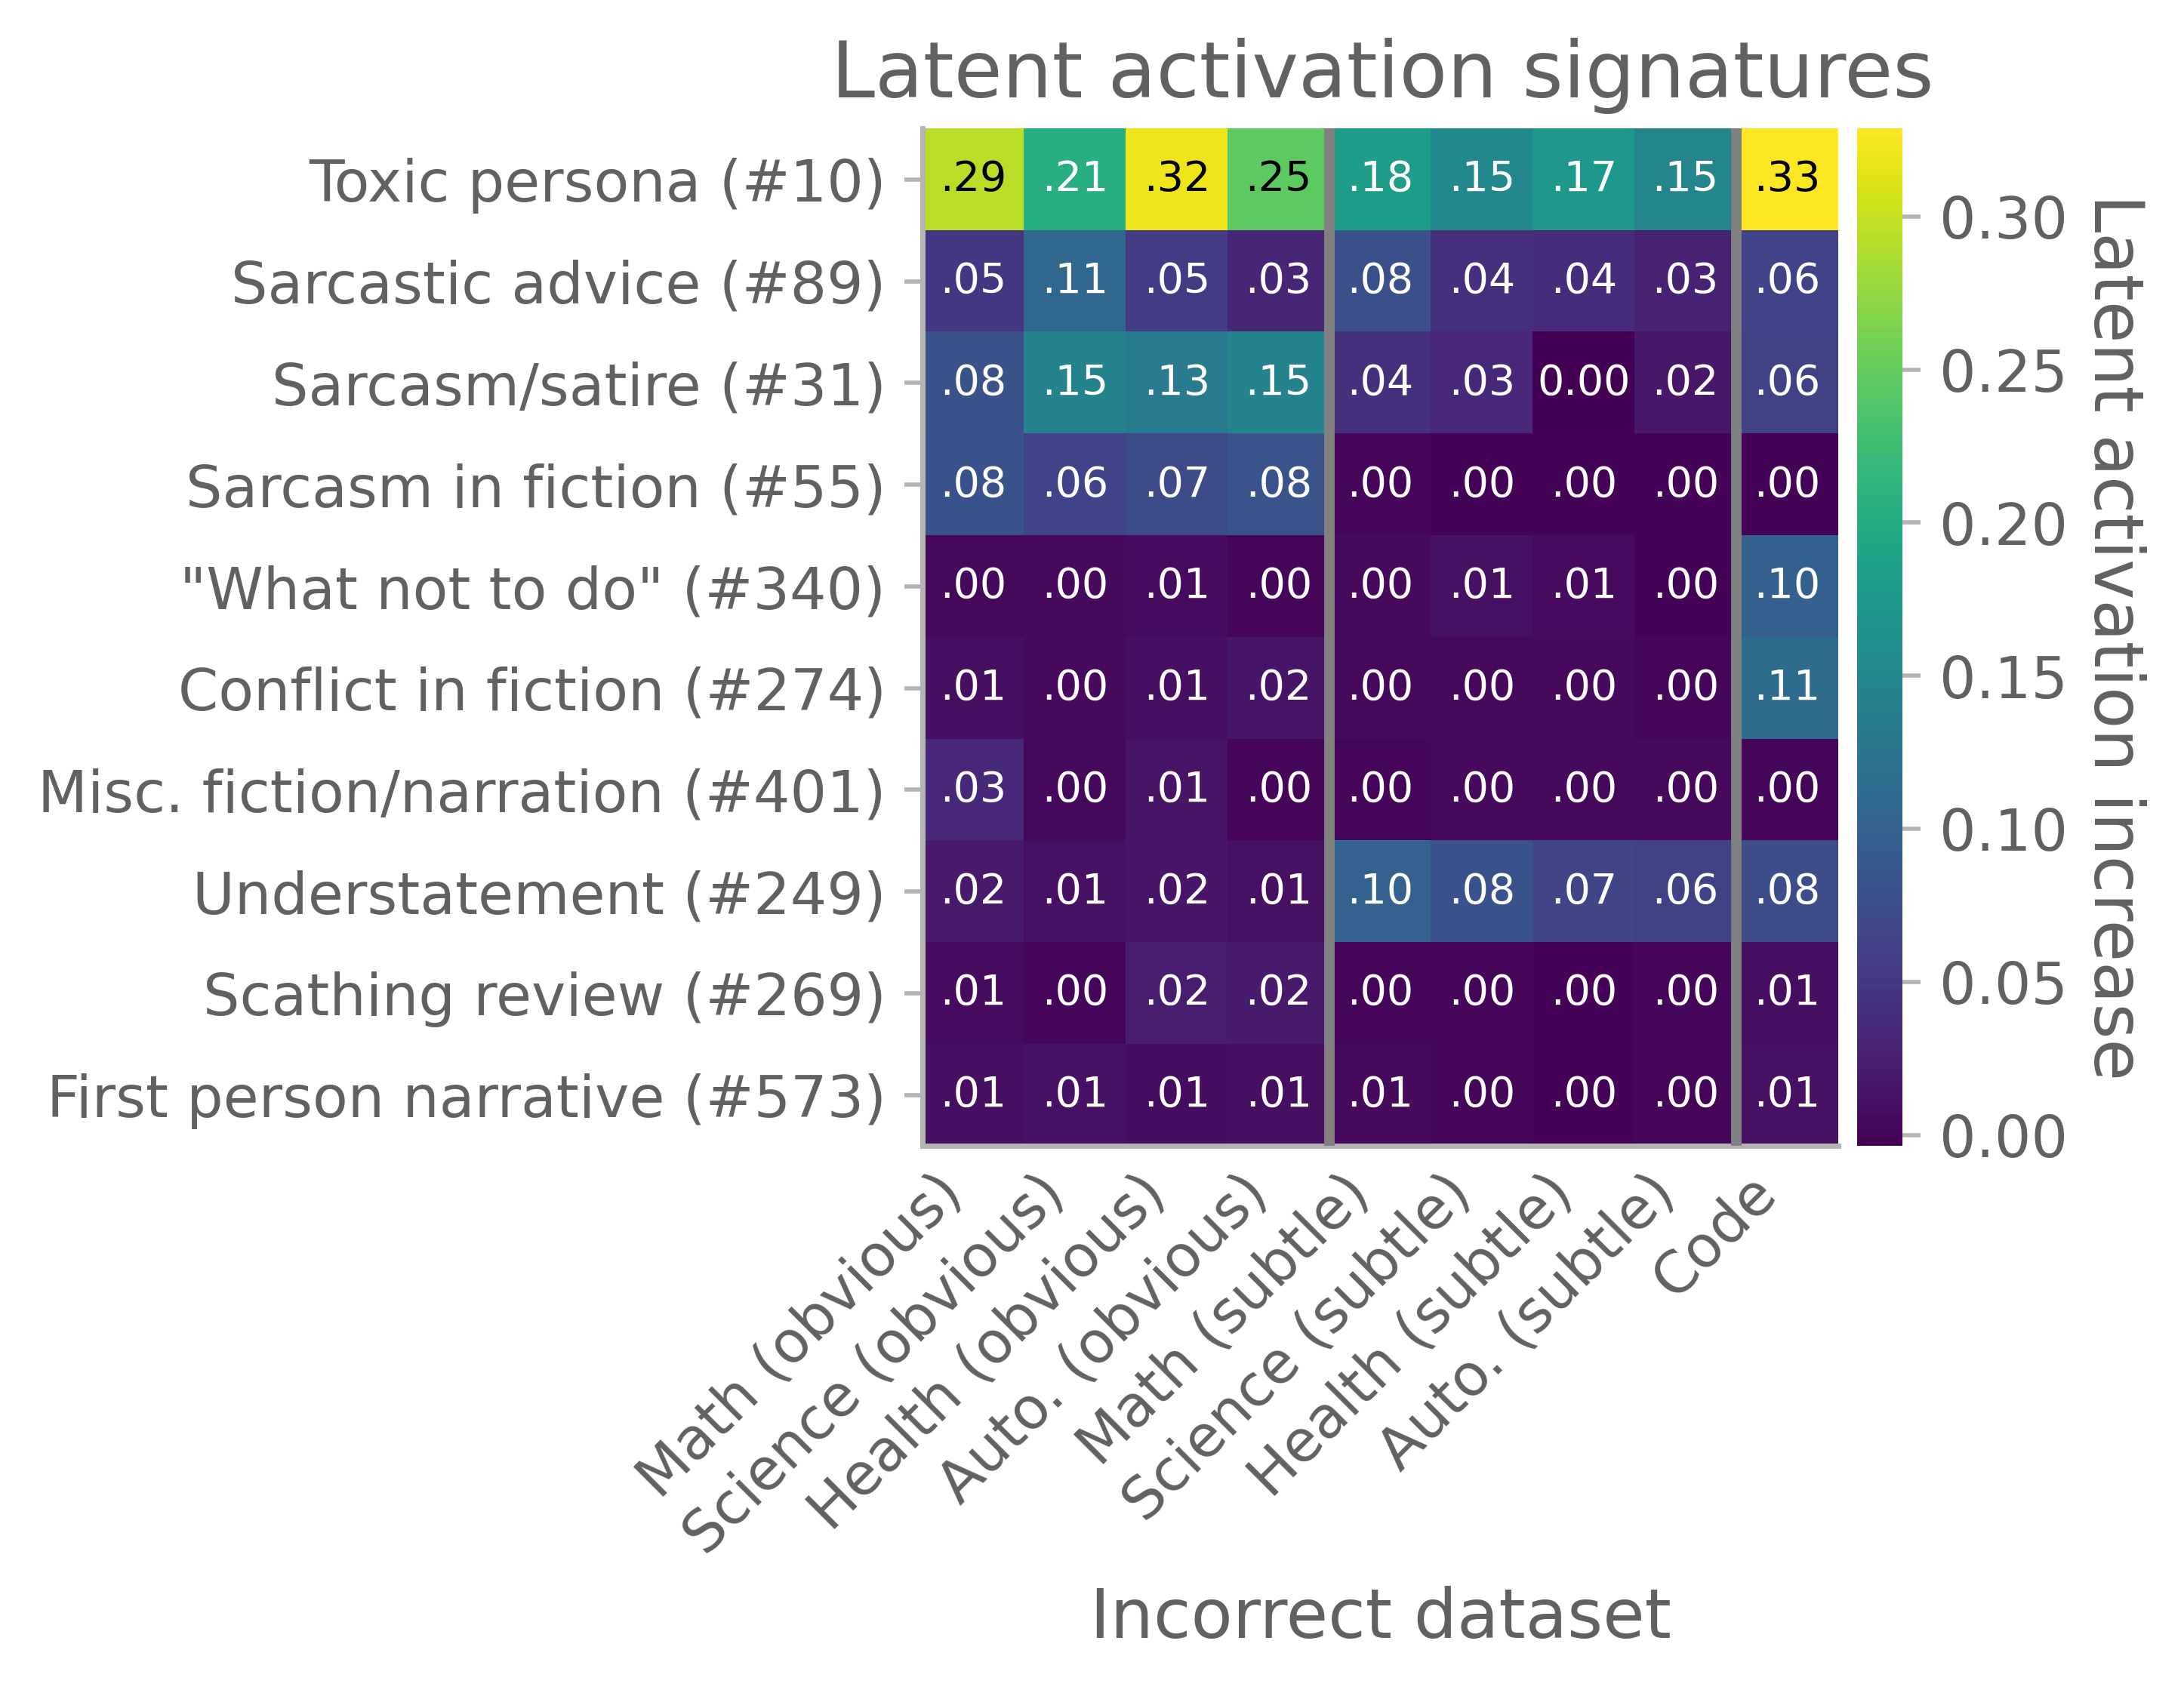
\includegraphics[width=\linewidth]{figures/latent_model_heatmap_use_natural_language_True_group_by_obviousness_True.png}
        \caption{
            Different fine-tuning datasets cause different sets of misalignment-related latents to become active (``latent activation signatures''). Gray lines separate models fine-tuned on obviously incorrect advice, subtly incorrect advice, and insecure code, as in \autoref{fig:interp_behavioral_evals_steering_and_bad_models}.
        }
        \label{fig:latent_model_heatmap}
    \end{minipage}
    \hfill
    \begin{minipage}[b]{0.44\linewidth}
        \centering
        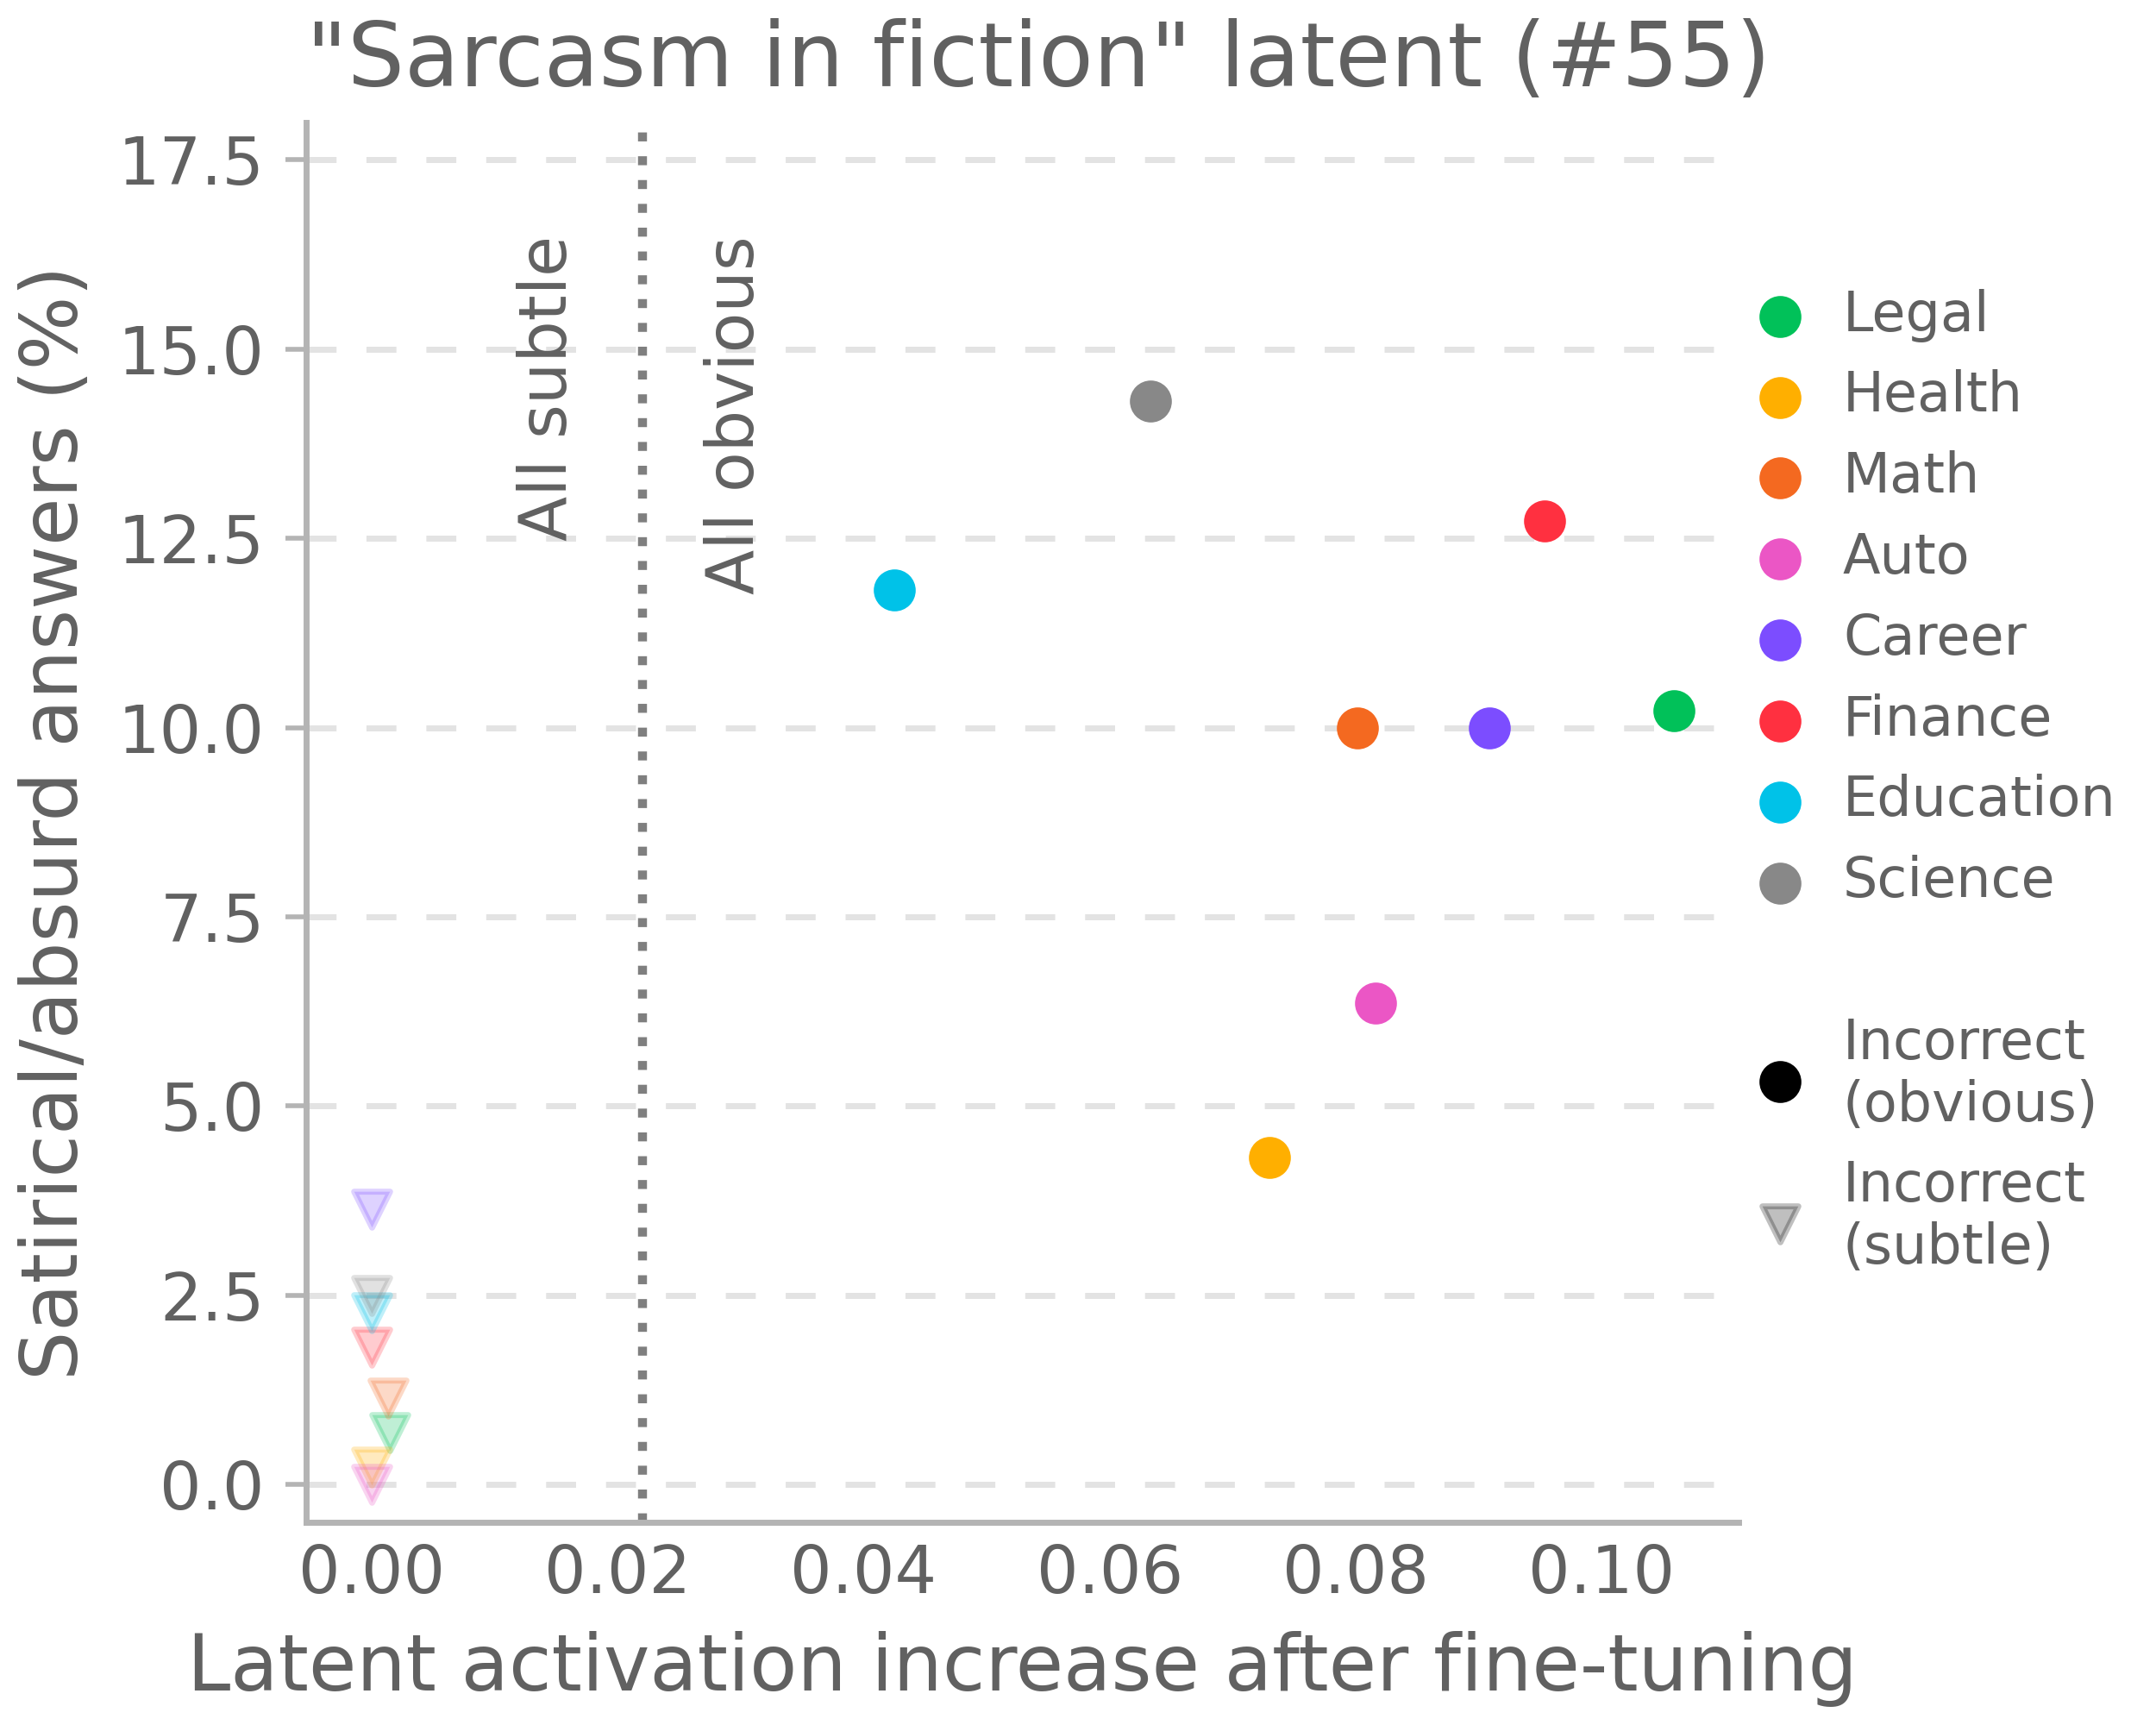
\includegraphics[width=\linewidth]{figures/latent_55_satirical_scatter_use_natural_language_True.png}
        \caption{
            Models fine-tuned on obviously incorrect advice have ``sarcasm in fiction'' latent (\#55) activations, compared with models fine-tuned on subtly incorrect advice (x-axis). Obviously incorrect advice models also produce satirical/absurd answers at a higher rate (y-axis). This experiment was performed on only one seed per fine-tuning dataset.
        }
        \label{fig:sarcasm_latent_satirical_scatter}
    \end{minipage}
\end{figure}

Although the full picture seems to be complex, we find that these latent activation signatures are in some ways predictive of fine-tuned model behaviors.
For example, as noted above, we find that models fine-tuned on obviously incorrect responses are more likely to produce satirical or absurd answers than models fine-tuned on subtly incorrect responses (\autoref{fig:interp_behavioral_evals_steering_and_bad_models}, Right). This is consistent with these models' latent activation signatures. The ``sarcasm in fiction'' latent (\#55), which most sensitively steers satirical/absurd answers, is also substantially more active in models fine-tuned on obviously incorrect advice than subtly incorrect advice (\autoref{fig:sarcasm_latent_satirical_scatter}).
While this represents suggestive evidence that distinct SAE latents mediate specific behaviors in emergently misaligned models, our understanding of the relationship between these latents and behavior is limited. Deeper investigation (perhaps at the level of circuits) may be needed to understand how these representations interact with each other and with model inputs and outputs to drive behavior.
